Աշխատանքի երրորդ գլուխը նվիրված է միջակայքային ներկում չունեցող մուլտիգրաֆներին: Կամայական $G$ մուլտիգրաֆի համար $w_{def}(G)$-ով և $W_{def}(G)$-ով նշանակենք $t$-ի ամենափոքր և ամենամեծ արժեքները, որոնց համար $G$-ն ունի $\alpha$ ճիշտ կողային $t$-ներկում $def(G,\alpha)=def(G)$ դեֆիցիտով: Ալտինակարը, Կապորոսսին և Հերցը\footnote{H.S. Altinakar, G. Caporossi, A. Hertz, A comparison of integer and constraint programming models for the deficiency problem, Computers and Oper. Res. 68, 2016, pp. 89-96.} ցույց են տվել, որ եթե $|V(G)|\geq 3$, ապա $W_{def}(G)\leq 2\vert V(G)\vert -4+def(G)$: Երրորդ գլխի առաջին պարագրաֆում ապացուցվել են համանման գնահատականներ գրաֆների մի շարք դասերի համար:

\begin{theorem}
\label{t3_W_Wdef} Դիցուք $f:\mathbb{N} \rightarrow \mathbb{Z}$, իսկ $\mathfrak{C}$-ն գրաֆների որևէ փակ դաս է կախված կող ավելացնելու գործողության նկատմամբ: Եթե
$W(G^{\prime})\leq
f(\vert V(G^{\prime})\vert)$ պայմանը տեղի ունի կամայական $G^{\prime}\in
\mathfrak{C} \cap \mathfrak{N}$ գրաֆի համար, ապա ցանկացած $G\in \mathfrak{C}$ գրաֆի համար $W_{def}(G)\leq f\left(\vert V(G)\vert+def(G)\right)$
\end{theorem}
\begin{proof}[Ապացույց]
Դիցուք $G\in \mathfrak{C}$ և $\alpha$-ն $G$-ի ճիշտ կողային ներկում է $W_{def}(G)$ գույներով, ընդ որում $def(G,\alpha)=def(G)$:

Սահմանենք $G^{\prime}$ օժանդակ գրաֆը հետևյալ կերպ. կամայական $v\in V(G)$ գագաթի համար, որի համար $def(v,\alpha)>0$, $v$ գագաթից կախենք թվով $def(v,\alpha)$ նոր կողեր: Պարզ է, որ $G^{\prime}\in\mathfrak{C}$ և $\vert V(G^{\prime})\vert = \vert V(G)\vert +def(G)$: Այնուհետև, շարունակենք $G$-ի $\alpha$ $W_{def}(G)$ գույներով ճիշտ կողային ներկումը մինչև $G^{\prime}$-ի $\beta$ ճիշտ կողային ներկում $W_{def}(G)$ գույներով հետևյալ կերպ. կամայական $v\in V(G)$ գագաթի համար, որի համար $def(v,\alpha)>0$, ներկենք $v$-ին նոր ավելացված կողերը $\left[\underline
S\left(v,\alpha \right),\overline S\left(v,\alpha
\right)\right]\setminus S(v,\alpha)$ բազմության տարբեր գույներով: $\beta$-ի սահմանման և $G^{\prime}$-ի կառուցման համաձայն կստանանք, որ $G^{\prime}$-ը ունի միջակայքային $W_{def}(G)$-ներկում: Քանի որ $G^{\prime}\in \mathfrak{C}\cap\mathfrak{N}$, ունենք, որ
\begin{center}
$W_{def}(G)\leq W(G^{\prime})\leq f(\vert V(G^{\prime})\vert)= f\left(\vert V(G)\vert+def(G)\right)$:
\end{center}
\end{proof}

Այս թեորեմից մասնավորապես հետևում է, որ եթե $G$-ն եռանկյուն չպարունակող գրաֆ է, ապա
$W_{def}(G)\leq \vert V(G)\vert +def(G)-1$: Կատարյալ զուգակցում չունեցող գրաֆների $w_{def}(G)$-ի համար ստացվել է ստորին գնահատական, որն ընդհանրացնում է Հետևանք \ref{c1_lower_nopm}-ը:
\begin{hide}
\begin{corollary}
\label{c3_Wdef_notriangle} Եթե $G$-ն եռանկյուն չպարունակող գրաֆ է, ապա
$W_{def}(G)\leq \vert V(G)\vert +def(G)-1$:
\end{corollary}

\begin{corollary}
\label{c3_Wdef_bipartite} Եթե $G$-ն երկկողմանի գրաֆ է, ապա
$W_{def}(G)\leq \vert V(G)\vert +def(G)-1$:
\end{corollary}

\begin{corollary}
\label{c3_Wdef_planar} Եթե $G$-ն հարթ գրաֆ է, ապա
$W_{def}(G)\leq \frac{11}{6}\left(\vert V(G)\vert +def(G)\right)$:
\end{corollary}
\end{hide}

\begin{hide}
\begin{theorem}
\label{t3_Wdef_paths} Եթե $G$-ն կապակցված գրաֆ է, ապա
\begin{center}
$W_{def}(G)\leq 1+def(G)+{\max\limits_{P\in
\mathbf{P}}}{\sum\limits_{v\in V(P)}}\left(d_{G}(v)-1\right)$,
\end{center}
որտեղ $\mathbf{P}$-ն $G$-ի բոլոր կարճագույն շղթաների բազմությունն է:
\end{theorem}
\begin{proof}[Ապացույց] Ապացույցում կհետևենք \cite{AsratianKamalian1994}-ում Թեորեմ 2-ի ապացույցի սխեմային:
Դիցուք $\alpha$-ն $G$-ի ճիշտ ներկում է $W_{def}(G)$ գույներով, ընդ որում $def(G,\alpha)=def(G)$:

Թեորեմ \ref{t3_W_Wdef}-ի ապացույցին համանման սահմանենք $H$ օժանդակ գրաֆը $H$ հետևյալ կերպ. ցանկացած $v\in V(G)$ գագաթի համար, որի համար $def(v,\alpha)>0$, $v$ գագաթին ավելացնենք թվով $def(v,\alpha)$ կախված կողեր: Պարզ է, որ $H$-ը կապակցված գրաֆ է: 
$G$-ի $\alpha$ ճիշտ ներկումը $W_{def}(G)$ գույներով շարունակենք մինչև $H$-ի $\beta$ ճիշտ ներկում $W_{def}(G)$ գույներով հետևյալ կերպ.
կամայական $v\in V(G)$ գագաթի համար, որի համար $def(v,\alpha)>0$, $v$-ին կից ավելացված կողերը ներկենք $\left[\underline
S\left(v,\alpha \right),\overline S\left(v,\alpha
\right)\right]\setminus S(v,\alpha)$ բազմության տարբեր գույներով: Ըստ $\beta$-ի սահմանման և $H$-ի կառուցման ստանում ենք, որ $H$-ը ունի միջակայքային
$W_{def}(G)$-ներկում: $H$-ի $\beta$ ներկման մեջ դիտարկենք $1$ և $W_{def}(G)$ գույներով ներկված կողերը: Դիցուք, $e=u_{1}u_{2},
e^{\prime}=w_{1}w_{2}$ և $\beta(e)=1,
\beta(e^{\prime})=W_{def}(G)$: Առանց ընդհանրությունը խախտելու, կարող ենք ենթադրել, որ $e$-ն և $e^{\prime}$-ը միացնող $P$ կարճագույն շղթան միացնում է 
$u_{1}$ և $w_{1}$ գագաթները, որտեղ $P=v_{0}e_{1}v_{1}\ldots
v_{i-1}e_{i}v_{i}\ldots v_{k-1}e_{k}v_{k}$ և $v_{0}=u_{1}$,
$v_{k}=w_{1}$:

Քանի որ $\beta$-ն $H$-ի միջակայքային $W_{def}(G)$-ներկում է, ունենք, որ

\begin{center}
$\beta(e_{1})\leq d_{H}(v_{0})$,

$\beta(e_{2})\leq \beta(e_{1})+d_{H}(v_{1})-1$,

$\cdots \cdots \cdots \cdots \cdots \cdots$

$\beta(e_{i})\leq \beta(e_{i-1})+d_{H}(v_{i-1})-1$,

$\cdots \cdots \cdots \cdots \cdots \cdots$

$\beta(e_{k})\leq \beta(e_{k-1})+d_{H}(v_{k-1})-1$,

$\beta(e^{\prime})\leq \beta(e_{k})+d_{H}(v_{k})-1$.

\end{center}

Գումարելով այս անհավասարությունները, կստանանք.

\begin{center}
$\beta(e^{\prime})\leq 
1+{\sum\limits_{j=0}^{k}\left(d_{H}(v_{j})-1\right)}$:
\end{center}

Այստեղից ստանում ենք, որ
\begin{eqnarray*}
W_{def}(G)=\beta(e^{\prime}) &\leq&
1+{\sum\limits_{j=0}^{k}\left(d_{H}(v_{j})-1\right)}\leq
1+def(G)+{\sum\limits_{j=0}^{k}\left(d_{G}(v_{j})-1\right)}\\
&\leq& 1+def(G)+{\max\limits_{P\in \mathbf{P}}}{\sum\limits_{v\in
V(P)}}\left(d_{G}(v)-1\right):
\end{eqnarray*}
\end{proof}

\begin{corollary}
\label{c3_Wdef_diam} Եթե $G$-ն կապակցված գրաֆ է, ապա
\begin{center}
$W_{def}(G)\leq
1+def(G)+(\mathrm{diam}(G)+1)\left(\Delta(G)-1\right)$:
\end{center}
\end{corollary}
\end{hide}

\begin{theorem}
\label{t3_wdef_nopm} Եթե $G$-ն չունի կատարյալ զուգակցում, ապա
$w_{def}(G)\geq 2\delta(G)-def(G)$:
\end{theorem}
\begin{proof}[Ապացույց] Այս թեորեմի ապացույցում մենք հետևում ենք \cite{BouchardHertzDesaulniers}-ի Պնդում 2-ի ապացույցին:

Դիցուք $\alpha$-ն $G$-ի ճիշտ ներկում է $w_{def}(G)$ գույներով և 
$def(G,\alpha)=def(G)$:

Հեշտ է տեսնել, որ ցանկացած $v\in V(G)$ գագաթի համար ունենք, որ

\begin{center}
$1\leq \underline S\left(v,\alpha \right)\leq
w_{def}(G)-\delta(G)+1$:
\end{center}

Ենթադրենք, որ $w_{def}(G)-\delta(G)+1\leq \delta(G)$ (հակառակ դեպքում՝
$w_{def}(G)\geq 2\delta(G)\geq 2\delta(G)-def(G)$):

Քանի որ $G$-ն չունի կատարյալ զուգակցում, կամայական $c\in
\left[w_{def}(G)-\delta(G)+1,\delta(G)\right]$ գույնի համար գոյություն ունի առնվազն մեկ գագաթ $v_{c}$ այնպիսին, որ $c\notin S\left(v_{c},\alpha\right)$
և $\underline S\left(v_{c},\alpha \right)<c<\overline
S\left(v_{c},\alpha \right)$: Այստեղից հետևում է, որ առնվազն
$2\delta(G)-w_{def}(G)$ գույներ բացակայում են $G$-ի գագաթներից: Ուստի,
$def(G)\geq 2\delta(G)-w_{def}(G)$:
\end{proof}

Այս թեորեմը ընդհանրացնում է Բուշարի, Հերցի և Դեսոլնյեի կողմից\footnote{M. Bouchard, A. Hertz, G. Desaulniers, Lower bounds and a tabu search algorithm for the minimum deficiency problem, J. Comb. Optim. 17, 2009, pp. 168-191.} ստացված արդյունքը, համաձայն որի, եթե $G$-ն կենտ թվով գագաթներ ունեցող գրաֆ է, ապա $w_{def}(G)\geq 2\delta(G)-def(G)$:

\begin{hide}
\begin{corollary}
\label{c3_wdef_odd}\cite{BouchardHertzDesaulniers} Եթե $G$-ն կենտ թվով գագաթներ ունեցող գրաֆ է, ապա $w_{def}(G)\geq 2\delta(G)-def(G)$:
\end{corollary}

\begin{corollary}
\label{c3_wdef_odd_regular}\cite{BouchardHertzDesaulniers} Եթե $G$-ն կենտ թվով գագաթներ ունեցող $r$-համասեռ գրաֆ է և $def(G)=\frac{r}{2}$, ապա
$w_{def}(G)\geq \frac{3r}{2}$:
\end{corollary}
\end{hide}

Քամալյանը ապացուցել է, որ կամայական $l\in \mathbb{N}$ թվի համար գոյություն ունի $G$ գրաֆ այնպիսին, որ $G\in \mathfrak{N}$ և $W(G)-w(G)\geq l$: Հաջորդ թեորեմն ընդլայնում է այս արդյունքը դրական դեֆիցիտով գրաֆների համար:
\begin{theorem}
\label{t3_Wdef_wdef_difference} Ցանկացած $l\in \mathbb{N}$ թվի համար գոյություն ունի $G$ գրաֆ այնպիսին, որ $def(G)>0$ և $W_{def}(G)-w_{def}(G)\geq l$:
\end{theorem}
\begin{proof}[Ապացույց]
Դիցուք $p=2l+1$ և $G=K_{2p+1}$: Քանի որ $def(G)=p>0$ և $w_{def}(G)=3p$, ապա ապացույցը ավարտելու համար բավարար է ցույց տալ, որ $W_{def}(G) \geq 3p + \frac{p-1}{2} = 3p + l$: Մենք կապացուցենք փոքր ինչ ավելի ընդհանուր արդյունք բոլոր կենտ թվով գագաթներով լրիվ գրաֆների համար: Ցույց կտանք, որ եթե $n = p2^q$, որտեղ $p$-ն կենտ է, իսկ $q \in \mathbb{Z}_+$, ապա
\begin{center}
$W_{def}(K_{2n+1}) \geq 3n + \frac{p-1}{2}$:
\end{center}

\begin{figure}[t!]
\centering
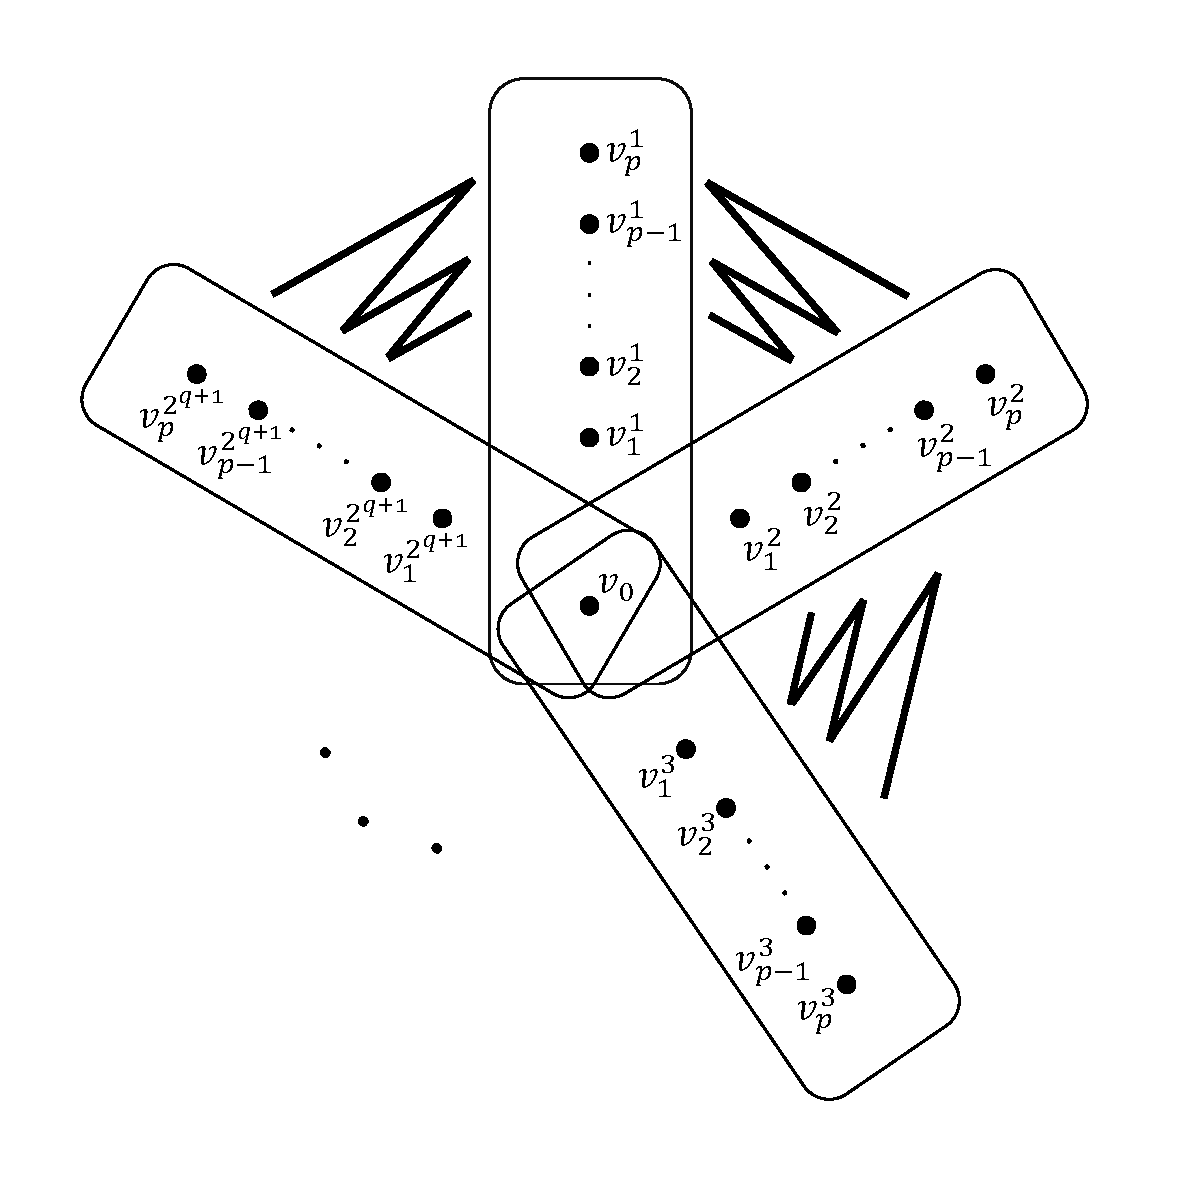
\includegraphics[width=0.7\textwidth]{figures/complete-graph-edges.pdf}
\caption{$K_{p2^{q+1}+1}$ գրաֆի գագաթները բաժանում ենք $2^{q+1}$ խմբերի այպես, որ կամայական երկու խմբի հատումը $v_0$ գագաթն է:}
\label{complete-graph}
\end{figure}

$K_{p2^{q+1}+1}$-ի $\phi$ կողային ներկումը կառուցենք օգտագործելով % compose !!!
տարբեր գրաֆների երեք ներկումներ:

\begin{enumerate}
    \item Մեզ հարկավոր է Թեորեմ \ref{tPetrosyan3n2}-ում նկարագրված $K_{p+1}$-ի $\alpha$ միջակայքային $\left(\frac{3}{2}(p+1)-2 \right)$-ներկումը: $K_{p+1}$-ի գագաթները նշանակենք հետևյալ կերպ. $V(K_{p+1}) = \{u_i : i=0, \ldots, p\}$: $\alpha$ ներկումը ունի մի կարևոր հատկություն, որ $\underline{S}(u_i, \alpha) = \lfloor \frac{i}{2} \rfloor + 1$ կամայական $i = 0,\ldots,p$ թվի համար:
    \item Այնուհետև, մեզ պետք է $K_{p,p}$-ի հատուկ տիպի ներկում, որը կնշանակենք $\beta$-ով: Դիցուք, $K_{p,p}$-ի գագաթներն են. $V(K_{p,p}) = \{x_i,y_i:i=1,\ldots,p\}$: $\beta$ ներկումը պետք է բավարարի հետևյալ պայմանին. կամայական $i=1,\ldots,p$ թվի համար $\underline{S}(x_i,\beta) = \underline{S}(y_i,\beta) = \left\lfloor \frac{i}{2} \right\rfloor + 1$: Այս պայմանին բավարարող $K_{p,p}$-ի ներկման գոյությունը հետևում է \cite{TepanyanPetrosyan} աշխատանքի Լեմմա 4-ից:
    \item Վերջապես, մեզ պետք է $K_{2^{q+1}+1}$ գրաֆի որևէ $\gamma$ ներկում $3\cdot2^q$ գույներով: Գրաֆի գագաթները նշանակենք $V(K_{2^{q+1}+1}) = \left\{w^j : j=0,\ldots, 2^{q+1} \right\}$: $\gamma$-ն պետք է բավարարի հետևյալ պայմանին. $def(K_{2^{q+1}+1},\gamma) = def(w^0, \gamma) = 2^q$: Այսպիսի հատկանիշներով ներկումներ նկարագրված են \cite{GiaroKubaleMalafiejski2001}-ի Թեորեմ 4.2-ում և \cite{PetrosyanMkhitaryan}-ի Թեորեմ 29-ում:
\end{enumerate}


$K_{p2^{q+1}+1}$ գրաֆի գագաթները նշանակենք հետևյալ կերպ (Նկ. \ref{complete-graph}). 
\begin{align*}
V\left(K_{p2^{q+1}+1}\right) = \{v_0\} \cup \left\{v_i^j : i=1,\ldots,p,\ j=1,\ldots,2^{q+1} \right\}.
\end{align*}

Կառուցենք նրա $\phi$ ներկումը հետևյալ կերպ.
\begin{align*}
\phi\left(v_{i_1}^j v_{i_2}^j\right) &= \alpha(u_{i_1}u_{i_2}) + p\left(\gamma(w^0w^j) - 1\right), & 0 \leq i_1 < i_2 \leq p, & & 1 \leq j \leq 2^{q+1}, \\
\phi\left(v_{i_1}^{j_1}v_{i_2}^{j_2}\right) &= \beta(x_{i_1}y_{i_2}) + p\left(\gamma(w^{j_1}w^{j_2}) - 1\right), & 1 \leq i_1, i_2 \leq p, & & 1 \leq j_1 < j_2 \leq 2^{q+1}: 
\end{align*} % !!! հայատառ վերջակետ

Վերևում բերված բանաձևերում $v_0^j$ սիմվոլները վերաբերվում են միևնույն $v_0$ գագաթին, % !!!!
կամայական $j=1,\ldots,2^{q+1}$ թվի համար: % !! թվի համար
Առաջին բանաձևը ներկում է այն կողերը, որոնց ծայրակետերը պատկանում են Նկ. \ref{complete-graph}-ում միևնույն խմբին, մինչդեռ երկրորդ բանաձևը ներկում է այն կողերը, որոնք միացնում են տարբեր խմբերին պատկանող գագաթները: Ցույց տանք, որ $v_i^j$, $i=1,\ldots,p$, $j=1,\ldots,2^{q+1}$, գագաթների սպեկտրները միջակայքեր են:
\begin{align*}
    S\left(v^j_i,\phi\right) &= \left[\underline{S}(u_i, \alpha) + p\left(\gamma(w^0w^j) - 1\right), \overline{S}(u_i, \alpha) + p\left(\gamma(w^0w^j) - 1\right)\right] \\
    &\cup \bigcup\limits_{j'\in [1, 2^{q+1}] \setminus \{j\}}{\left[\underline{S}(x_i, \beta) + p\left(\gamma(w^jw^{j'}) - 1\right), \overline{S}(x_i, \beta) + p\left(\gamma(w^jw^{j'}) - 1\right) \right]}.
\end{align*}
Ունենք, որ $\underline{S}(u_i, \alpha) = \underline{S}(x_i, \beta) = \lfloor \frac{i}{2} \rfloor + 1$ կամայական $i = 1,\ldots,p$ թվի համար: % Թվի համար
Ուստի վերը նշված արտահայտությունը դառնում է.
\begin{align*}
    S\left(v^j_i,\phi\right) &= \left[\left\lfloor \frac{i}{2} \right\rfloor + 1 + p\left(\gamma(w^0w^j) - 1\right), \left\lfloor \frac{i}{2} \right\rfloor + p + p\left(\gamma(w^0w^j) - 1\right)\right] \\
    &\cup \bigcup\limits_{j'\in [1, 2^{q+1}] \setminus \{j\}}{\left[\left\lfloor \frac{i}{2} \right\rfloor + 1 + p\left(\gamma(w^jw^{j'}) - 1\right), \left\lfloor \frac{i}{2} \right\rfloor + p + p\left(\gamma(w^jw^{j'}) - 1\right) \right]}\\
    &= \bigcup\limits_{j'\in [0, 2^{q+1}] \setminus \{j\}}{\left[\left\lfloor \frac{i}{2} \right\rfloor + 1 + p\left(\gamma(w^jw^{j'}) - 1\right), \left\lfloor \frac{i}{2} \right\rfloor + p + p\left(\gamma(w^jw^{j'}) - 1\right) \right]}\\
    &= \left[\left\lfloor \frac{i}{2} \right\rfloor + 1 + p\left(\underline{S}(w^j,\gamma) - 1\right), \left\lfloor \frac{i}{2} \right\rfloor + p + p\left(\overline{S}(w^j,\gamma) - 1\right) \right]:
\end{align*}
Վերջին հավասարությունը տեղի ունի, քանի որ $S\left(w^j, \gamma\right)$ սպեկտրը միջակայք է բոլոր $j=1,\ldots,2^{q+1}$ թվերի համար: Վերջապես, $v_0$-ի սպեկտրը և $\phi$ ներկման դեֆիցիտը $v_0$ գագաթում կլինեն.
\begin{align*}
    S\left(v_0,\phi\right) &= \bigcup\limits_{j'\in [1, 2^{q+1}]} {\left[ \underline{S}(u_0, \alpha) + p\left(\gamma(w^0w^{j'}) - 1\right), \overline{S}(u_0, \alpha) + p\left(\gamma(w^0w^{j'}) - 1\right) \right]}\\
    &= \bigcup\limits_{j'\in [1, 2^{q+1}]} {\left[ 1 + p\cdot\gamma(w^0w^{j'}) - p, p\cdot\gamma(w^0w^{j'}) \right]},\\
    def(v_0, \phi) &= \overline{S}(v_0, \phi) - \underline{S}(v_0, \phi)-d_{K_{2n+1}}(v_0) + 1\\
    &= p\cdot\overline{S}(w^0,\gamma) - (1 + p\cdot\underline{S}(w^0,\gamma) - p)-p\cdot2^{q+1} + 1\\
    &= p\left(\overline{S}(w^0,\gamma) - \underline{S}(w^0,\gamma)-d_{K_{2^{q+1}+1}}(w^0) + 1\right) = p\cdot def(w^0,\gamma) = p2^q = n:
\end{align*}

Դիցուք $w^{\underline{j}}$ և $w^{\overline{j}}$ $K_{2^{q+1}+1}$-ի այն գագաթներն են, որոնց համար $\underline{S}\left(w^{\underline{j}}, \gamma\right) = 1$ և $\overline{S}\left(w^{\overline{j}}, \gamma\right) = 3\cdot2^q$: Հեշտ է տեսնել, որ $\underline{S}\left(v^{\underline{j}}_{1},\phi\right) = 1$ և $\overline{S}\left(v^{\overline{j}}_{p},\phi\right) = \left\lfloor \frac{p}{2} \right\rfloor + p + p\left(3\cdot2^q - 1\right) = 3n + \frac{p-1}{2}$: Ուստի, $\phi$-ն $K_{2n+1}$-ի ճիշտ կողային ներկում է $3n + \frac{p-1}{2}$ գույներով, ընդ որում $def(K_{2n+1}, \phi) = def\left(v_0, \phi\right) = n$:
\end{proof}

Հայտնի է, որ եթե $G$-ն համասեռ մուլտիգրաֆ է, $G \in \mathfrak{N}$, իսկ $w(G) \leq t \leq W(G)$, ապա $G$-ն ունի միջակայքային $t$-ներկում: Հաջորդ թեորեմն ընդլայնում է այս արդյունքը դրական դեֆիցիտով մուլտիգրաֆների համար:

\begin{theorem}
\label{t3_middle_colors_def}
Դիցուք $\alpha_0$-ն $G$ համասեռ մուլտիգրաֆի ճիշտ ներկում է $t_0$ գույներով, իսկ $D \subseteq V(G)$ նրա գագաթների որևէ ենթաբազմություն է: Եթե կամայական $v \in V(G) \setminus D$ գագաթի համար $def(v,\alpha_0)=0$, ապա ցանկացած $t$ թվի համար, $\overline{S}(D,\alpha_0) - \underline{S}(D,\alpha_0) + 1 \leq t \leq t_0$, $G$-ն ունի $\alpha$ ճիշտ $t$-ներկում այնպես, որ $def(v,\alpha) = def(v,\alpha_0)$ կամայական $v\in V(G)$ գագաթի համար:
\end{theorem}
\begin{proof}[Ապացույց]
Դիցուք $a = \underline{S}(D,\alpha_0) - 1$ և $b = t_{0} - \overline{S}(D,\alpha_0)$: Փաստացի $[\underline{S}(D,\alpha_0),\overline{S}(D,\alpha_0)]$ միջակայքից դուրս ունենք $a+b$ գույներ, և պետք է ազատվել դրանցից $(t_0 - t)$-ից: Կառուցենք $G$-ի $\alpha$ ճիշտ կողային ներկումը՝ վերցնելով բոլոր կողերի գույները $\alpha_0$ ներկումից և ապա փոփոխելով դրանց մի մասը: Նախ կփորձենք ազատվել $\overline{S}(D,\alpha_0)$-ից մեծ գույներից, և եթե դա բավարար չլինի, կազատվենք $\underline{S}(D,\alpha_0)$-ից փոքր գույներից: 

Եթե $t_0 - t \leq b$, ապա կամայական $e\in E(G)$ կողի համար, որի համար $\alpha_0(e)\in \left[t + 1, t_0\right]$, նշանակենք $\alpha(e) = \alpha_0(e) - \Delta(G)$:

Եթե $t_0 - t > b$, ապա կամայական $e\in E(G)$ կողի համար, որի համար $\alpha_0(e)\in \left[\overline{S}(D, \alpha_0) + 1, t_0\right]$, նշանակենք $\alpha(e) = \alpha_0(e) - \Delta(G)$: Այնուհետև, կամայական $e\in E(G)$ կողի համար, որի համար $\alpha_0(e)\in \left[1, t_0 - t - b \right]$, նշանակենք $\alpha(e) = \alpha_0(e) + \Delta(G)$:
Երկու դեպքերում էլ $D$ բազմության գագաթների սպեկտրները չեն փոփոխվում, իսկ մյուս գագաթների սպեկտրները մնում են միջակայքեր: Եթե $\underline{S}(V(G), \alpha) > 1$, ապա վերջնական ներկումը ստանալու համար բոլոր կողերի գույներից հանում ենք  $\underline{S}(V(G), \alpha) - 1$:
\end{proof}


\begin{hide}
\begin{corollary}
\label{c3_complete_odd_colors}
Դիցուք $n=p2^q$, որտեղ $p$-ն կենտ է, իսկ $q \in \mathbb{Z}_+$: Կամայական $t$ թվի համար, $3n \leq t \leq 3n + \frac{p-1}{2}$, $K_{2n+1}$-ը ունի $\alpha$ ճիշտ ներկում $t$ գույներով այնպես, որ $def(K_{2n+1},\alpha)=n$:
\end{corollary}
\begin{proof}[Ապացույց] Բավական է վերցնել Թեորեմ \ref{t3_Wdef_wdef_difference}-ի ապացույցում նկարագրված $K_{2n+1}$-ի $\alpha_0$ ճիշտ կողային ներկումը $\left(3n + \frac{p-1}{2}\right)$ գույներով, վերցնել $D=\{v_0\}$, որտեղ $v_0\in V(K_{2n+1})$ և $def(v_0,\alpha_0)=def(K_{2n+1},\alpha_0)=n$, և հաշվի առնել, որ $\overline{S}(D,\alpha_0) - \underline{S}(D,\alpha_0) + 1=\overline{S}(v_0,\alpha_0) - \underline{S}(v_0,\alpha_0) + 1= def(v_0,\alpha_0)+d_{K_{2n+1}}(v_0) =n+2n =3n$:
\end{proof}
\end{hide}